%%%%%%%%%%%%%%%%%%%%%%%%%%%%%%%%%%%%%%%%%
% Journal Article
% LaTeX Template
% Version 1.4 (15/5/16)
%
% This template has been downloaded from:
% http://www.LaTeXTemplates.com
%
% Original author:
% Frits Wenneker (http://www.howtotex.com) with extensive modifications by
% Vel (vel@LaTeXTemplates.com)
%
% License:
% CC BY-NC-SA 3.0 (http://creativecommons.org/licenses/by-nc-sa/3.0/)
%
%%%%%%%%%%%%%%%%%%%%%%%%%%%%%%%%%%%%%%%%%

%----------------------------------------------------------------------------------------
%	PACKAGES AND OTHER DOCUMENT CONFIGURATIONS
%----------------------------------------------------------------------------------------

\documentclass[twoside,twocolumn]{article}


\usepackage[
backend=biber,
style=alphabetic,
sorting=ynt
]{biblatex}

\addbibresource{main.bib}

\usepackage{url}
\usepackage{blindtext} % Package to generate dummy text throughout this template

\usepackage[sc]{mathpazo} % Use the Palatino font
\usepackage[T1]{fontenc} % Use 8-bit encoding that has 256 glyphs
\linespread{1.05} % Line spacing - Palatino needs more space between lines
\usepackage{microtype} % Slightly tweak font spacing for aesthetics

\usepackage[english]{babel} % Language hyphenation and typographical rules

\usepackage[hmarginratio=1:1,top=32mm,columnsep=20pt]{geometry} % Document margins
\usepackage[hang, small,labelfont=bf,up,textfont=it,up]{caption} % Custom captions under/above floats in tables or figures
\usepackage{booktabs} % Horizontal rules in tables

\usepackage{lettrine} % The lettrine is the first enlarged letter at the beginning of the text

\usepackage{enumitem} % Customized lists
\setlist[itemize]{noitemsep} % Make itemize lists more compact

\usepackage{abstract} % Allows abstract customization
\renewcommand{\abstractnamefont}{\normalfont\bfseries} % Set the "Abstract" text to bold
\renewcommand{\abstracttextfont}{\normalfont\small\itshape} % Set the abstract itself to small italic text

\usepackage{titlesec} % Allows customization of titles
\renewcommand\thesection{\Roman{section}} % Roman numerals for the sections
\renewcommand\thesubsection{\roman{subsection}} % roman numerals for subsections
\titleformat{\section}[block]{\large\scshape\centering}{\thesection.}{1em}{} % Change the look of the section titles
\titleformat{\subsection}[block]{\large}{\thesubsection.}{1em}{} % Change the look of the section titles

\usepackage{fancyhdr} % Headers and footers
\pagestyle{fancy} % All pages have headers and footers
\fancyhead{} % Blank out the default header
\fancyfoot{} % Blank out the default footer
\fancyhead[C]{Running title $\bullet$ May 2016 $\bullet$ Vol. XXI, No. 1} % Custom header text
\fancyfoot[RO,LE]{\thepage} % Custom footer text

\usepackage{titling} % Customizing the title section

\usepackage{hyperref}
\usepackage{graphicx} % For hyperlinks in the PDF
\usepackage{subcaption}

%----------------------------------------------------------------------------------------
%	TITLE SECTION
%----------------------------------------------------------------------------------------

\setlength{\droptitle}{-4\baselineskip} % Move the title up

\pretitle{\begin{center}\Huge\bfseries} % Article title formatting
\posttitle{\end{center}} % Article title closing formatting
\title{Article Title} % Article title
\author{%
\textsc{John Smith}\thanks{A thank you or further information} \\[1ex] % Your name
\normalsize University of California \\ % Your institution
\normalsize \href{mailto:john@smith.com}{john@smith.com} % Your email address
%\and % Uncomment if 2 authors are required, duplicate these 4 lines if more
%\textsc{Jane Smith}\thanks{Corresponding author} \\[1ex] % Second author's name
%\normalsize University of Utah \\ % Second author's institution
%\normalsize \href{mailto:jane@smith.com}{jane@smith.com} % Second author's email address
}
\date{\today} % Leave empty to omit a date
\renewcommand{\maketitlehookd}{%
\begin{abstract}
\noindent
my abstract text
\end{abstract}
}

%----------------------------------------------------------------------------------------

\begin{document}

% Print the title
\maketitle

%----------------------------------------------------------------------------------------
%	ARTICLE CONTENTS
%----------------------------------------------------------------------------------------

\section{Introduction}

In the paper \cite[Investigating causal factors of shallow landslides in grassland regions of Switzerland]{zweifel_samarin_meusburger_alewell_2021} shallow landslides in Switzerland and there causal factors are investigated.
They are using the group lasso algorithm \cite{group_lasso} for estimating coefficients over a set of causal factors (called features from now on).
The coefficient can then be taken as an indicator of importance for each causal factor (note however that it only shows correlation not causation).
Different model instances of the group lasso are trained with bootstrapped data as well as cross validation over a grid (\cite[R package used]{blockCV}) to get different estimates for the coefficients as well as the performance of the model.
As performance measure the brier score is used.
Those estimates are later used to get confidence intervals (frequentist statistic).

In this study project we want to investigate the same data but with a bayesian statistics approach.
Rather than frequentist statistic confidence intervals we want to build bayesian statistic credible intervals.
Instead of running bootstrapping over cross validation with the group lasso, we use the Bayesian Group Lasso algorithm \cite{bayesian_group_lasso} to approximate the full distribution over the coefficients of the features directly.
The distribution, or samples from its approximation, can then be used to get the credible intervals.

During the study project a bug in the original code was found and fixed (See section TODO), the original experiments were repeated with slight differences which origin could not be explained (see section TODO)
and some additional experiments were made (see section TODO) inspired by discussions with a Lab Rotation happening in parallel during this study project.

Due to time concerns the Bayesian investigation was only applied to each site and not the full model containing all sites.
Also due to lagging support of the chosen software package the actual applied model is a Bayesian LDA with a Pascal Prior rather than a Bayesian Logistic Regression with a Pascal Prior.
The goal of investigating conditional distributions of the data (e.g. data points in a concrete slope range) was set up but never finished (see section Further work).

For the Bayesian LASSO the software package TODO was chosen.
Later this turned out to be a mistake, as this software package only supports Bayesian Linear Regression with a Pascal Prior rather than Bayesian LASSO (Bayesian Logistic Regression with a Pascal Prior).
Applying Linear Regression on binary class labels is equivalent to the LDA algorithm (See Fisher).
Therefore, we assume here that we do a Bayesian LDA with a Pascal Prior.
Note that we do not show here if (See Fisher) actually still holds in the Bayesian framework as well as the chosen prior, this is currently simply an assumption, due to not being able to prove or disprove it.
All here mentioned Bayesian results are therefore this form of a Bayesian LDA with a Pascal Prior model rather than the originaly planned Bayesian LASSO.

%------------------------------------------------

\section{Bug in the original paper}

During investigating the code of \cite{zweifel_samarin_meusburger_alewell_2021}, we found a bug in accumulating the model brier score results of the bootstrap runs.
The variable for accumulating the results of the cross validation (inner loop) is not reset each bootstrap iteration, which leads to the results of the first of $n$ bootstrap iteration being added $n$ times, the results of the second bootstrap iteration being added $n-1$ times and so on.
Therefore, some results are counted multiple times as individual results leading to a too confident confidence interval in the brier score in figure 9 in \cite{zweifel_samarin_meusburger_alewell_2021}.
The bug is quit evident when investigating the file sizes of the bootstrap runs, as shown in figure \ref{fig:bug_evidence}.

In Figure \ref{fig:bug_fix} we show the confident intervals of the brier score for each site as in the original paper, our reproduction with the bug as well as our reproduction without the bug.

The bug has no effect on the coefficient figure 7 in \cite{zweifel_samarin_meusburger_alewell_2021}, as the accumulating error was only done for the results used in figure 9.

\begin{figure*}
    \centering
  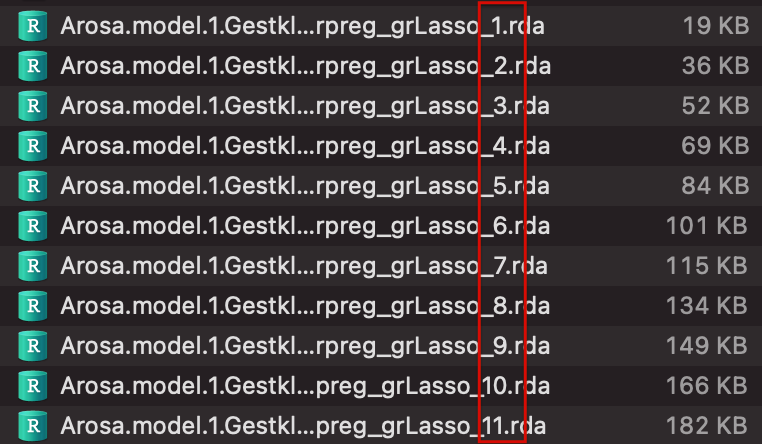
\includegraphics[width=\linewidth]{orig_filesize}
  \caption{File sizes of bootstrap run results. Red marked are the index of the bootstrap runs. We would expect that all file sizes are equal regardless of the index.}
  \label{fig:bug_evidence}
\end{figure*}

\begin{figure*}
    \centering
    \begin{subfigure}{.33\textwidth}
      \centering
      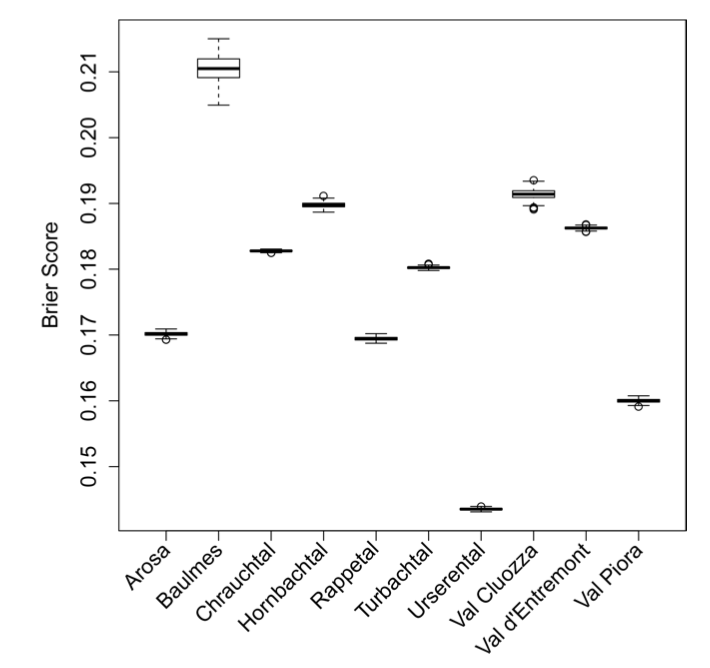
\includegraphics[width=\linewidth]{orig_brier_score}
      \caption{Original figure 9 in \cite{zweifel_samarin_meusburger_alewell_2021}}
      \label{fig:bug_fix:1}
    \end{subfigure}%
    \begin{subfigure}{.33\textwidth}
      \centering
      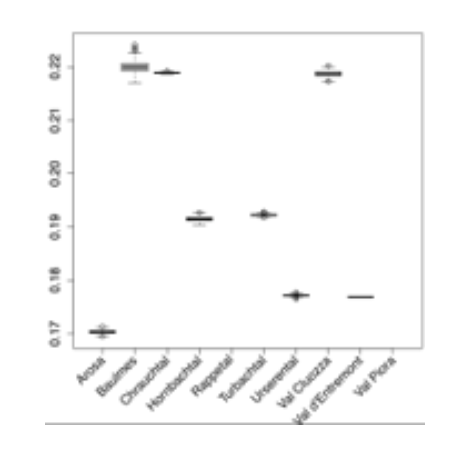
\includegraphics[width=\linewidth]{repr_brierscore_with_bug}
      \caption{Reproduction with bug}
      \label{fig:bug_fix:2}
    \end{subfigure}%
    \begin{subfigure}{.33\textwidth}
      \centering
      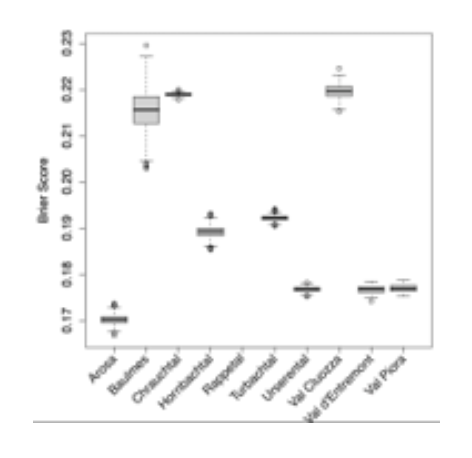
\includegraphics[width=\linewidth]{repr_brierscore}
      \caption{Reproduction with bug fix}
      \label{fig:bug_fix:3}
    \end{subfigure}
    \caption{(a) original paper (b) reproduction without bugfix. (c) reproduction with bugfix. \newline The bug caused duplication of samples therefore the confidence intervals was to narrow in the original paper. Some sites differ in reproduction (b) which cause was not found. }
    \label{fig:bug_fix}
\end{figure*}

\section{Reproducing results of original paper}

In figure \ref{fig:reproduction} we see the plot of the original paper as well as our reproduction.
In the reproduction variable the first dummy variable is removed otherwise the reproduction is the same as the original paper.

\begin{figure*}

    \centering

    \begin{subfigure}[b]{\textwidth}
       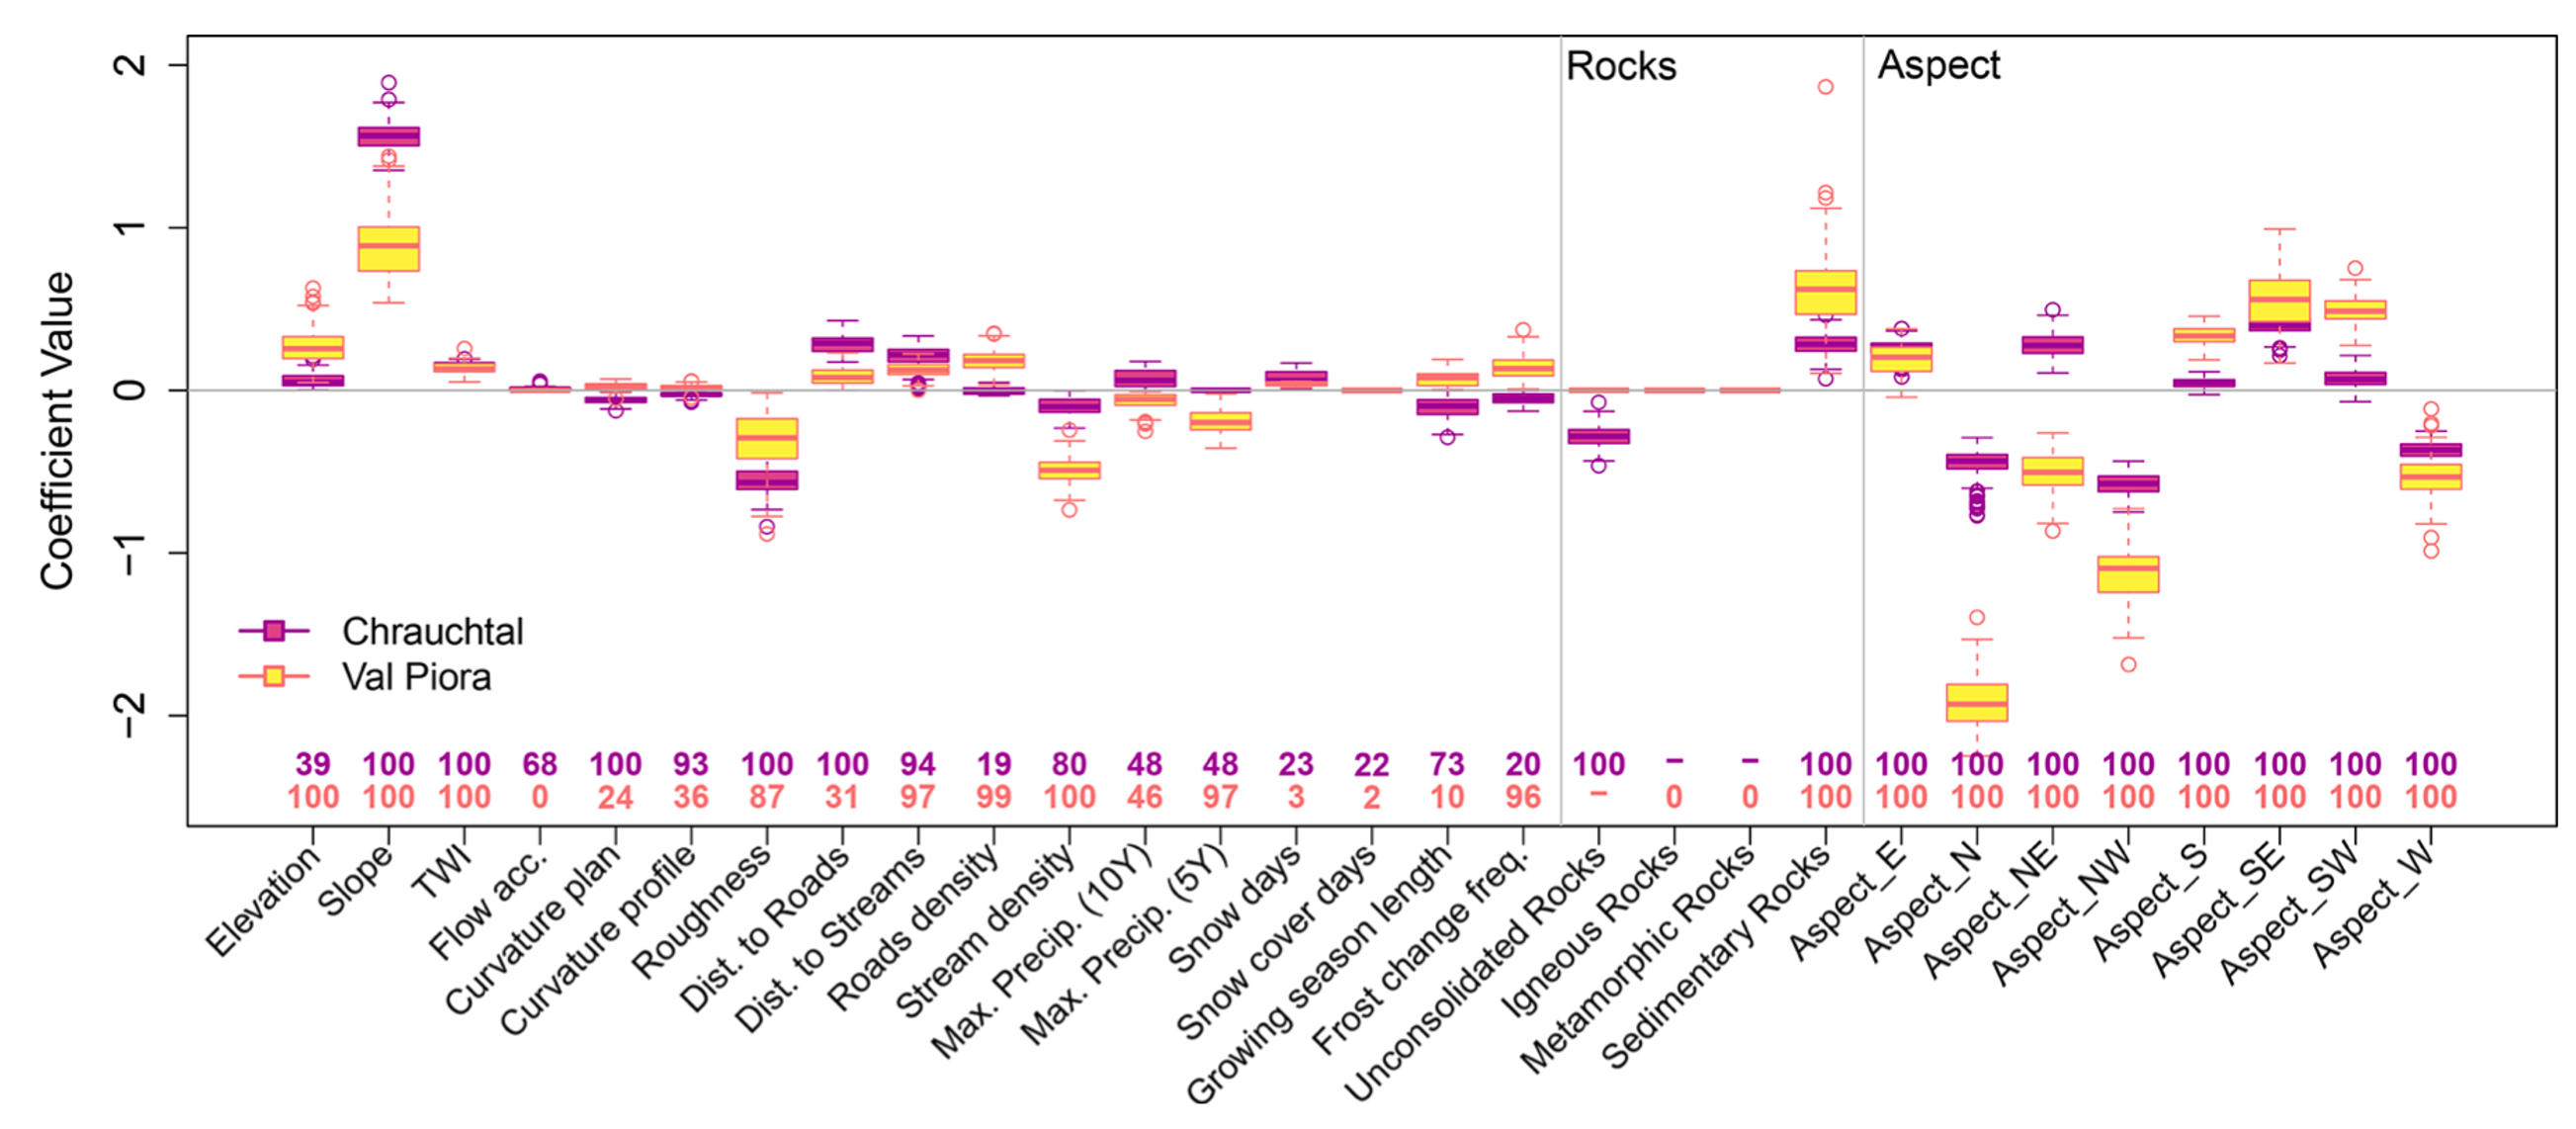
\includegraphics[width=1\textwidth]{orig_coef}
       \caption{Figure 7 from \cite{zweifel_samarin_meusburger_alewell_2021}}
       \label{fig:Ng1}
    \end{subfigure}

    \begin{subfigure}[b]{\textwidth}
       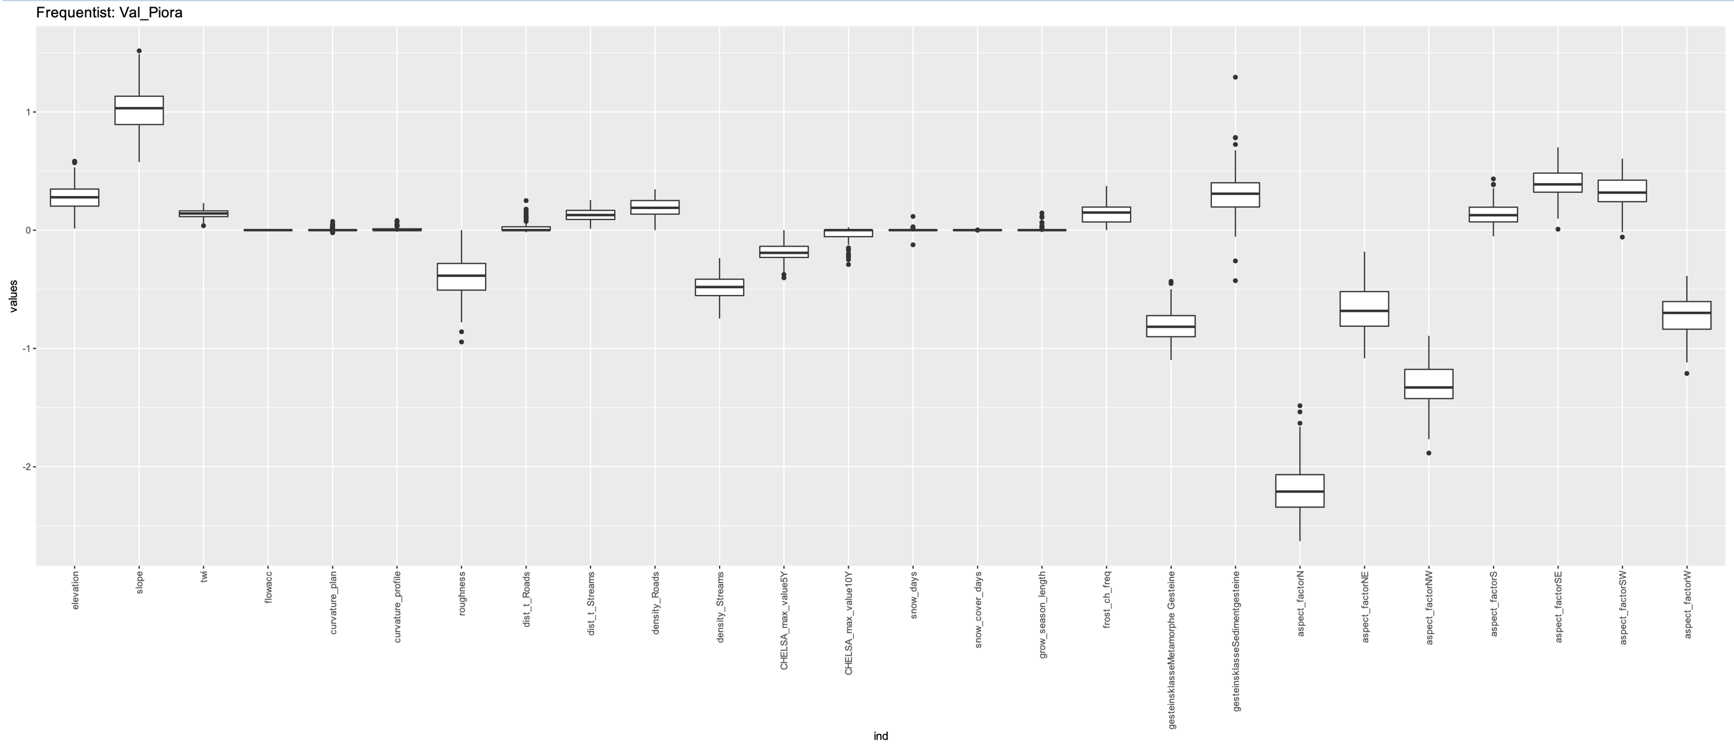
\includegraphics[width=1\textwidth]{rep_coef}
       \caption{Reproduction of coefficients from site Val Piora (yello boxplots from above figure)}
       \label{fig:Ng2}
    \end{subfigure}

    \caption[Two numerical solutions]{(a) Show the original plot from \cite{zweifel_samarin_meusburger_alewell_2021} as well as our (b) reproduction. Note that the reproduction seems to be correct. Only the categorical variables differ, which is explained as we drop the first dummy variable.}
    \label{fig:reproduction}
\end{figure*}

% The reproduction has unexplained differences that are not due to randomness as the seed is set as well as the gaps are probably to big for being only due to randomness.
% While reproducing the results we run into some problems due to different versions of R packages, maybe the difference has a similar cause.
% The actual cause was not found during the study project.

\section{Methods}

\subsection{Lasso}

\subsection{Frequentist Model}

\subsection{LDA}

\subsection{Bayesian Model}

\subsection{Differences}


\section{Results}

As in \cite{zweifel_samarin_meusburger_alewell_2021}

\section{Discussion}

TODO

%----------------------------------------------------------------------------------------
%	REFERENCE LIST
%----------------------------------------------------------------------------------------

\printbibliography

%----------------------------------------------------------------------------------------

\end{document}
